\newpage
\begin{center}
	\textbf{\large 3. РЕЗУЛЬТАТЫ}
\end{center}

\refstepcounter{chapter}
\addcontentsline{toc}{chapter}{3. РЕЗУЛЬТАТЫ}

\section{Результаты расчета захваченных частиц}

Приведем результаты численных расчетов для скорости захвата на Солнце для массы частицы темной материи $m_{\chi} = 100 \, \text{ГэВ}$. Рассмотрим вклад основных элементов в захват в зависимости от разницы масс $\delta$ (положительная $\delta$ означает эндотермическую реакцию, отрицательная --- экзотермическую). 
\begin{figure}[!h]
	\begin{center}
		\begin{tikzpicture}[scale=1]
			\begin{axis}[
				xscale = 1.7,
				yscale = 1.0,
				ymode = log,
				ymin = 1e-1,
				xlabel = $\delta \, \text{кэВ}$,
				xmax = 500,
				%xlabel shift = {(10,-10)},
				xtick distance=100,
				ylabel = $c^+_i$,
				legend style={at = {(0.56,0.08)},anchor = south,legend cell align=right}]
				\addplot [color = black, thick] table[x index=0,y index=7] {data/capture_rate_100GeV.txt};
				\addplot [color = red, thick] table[x index=0,y index=1] {data/capture_rate_100GeV.txt};
				\addplot [color = orange, thick] table[x index=0,y index=2] {data/capture_rate_100GeV.txt};
				\addplot [color = blue, thick] table[x index=0,y index=3] {data/capture_rate_100GeV.txt};
				\addplot [color = brown, thick] table[x index=0,y index=4] {data/capture_rate_100GeV.txt};
				\addplot [color = yellow, thick] table[x index=0,y index=5] {data/capture_rate_100GeV.txt};
				\addplot [color = cyan, thick] table[x index=0,y index=6] {data/capture_rate_100GeV.txt};
				\legend{Всего,H,He,Fe,O,N,Si}
			\end{axis}
		\end{tikzpicture}
		\caption{Вклад основных элементов в скорость захвата $c_+$ (\ref{capture_nd}) для Солнца при $m_{\chi} = 100 \, \text{ГэВ}$}
		\label{plot:fractions_sun_100GeV}
	\end{center}	
\end{figure}

Мы проверяли корректность расчетов, сравнивая эти доли с \cite{Blennow_2016}. 
Из графика видно, какие элементы дают наибольший вклад в захват. Так, при экзотермической реакции захват происходит в основном на гелии , как на втором по распространенности элементе (таблица \ref{tab:mass_fractions}), при этом водород играет незначительную роль в захвае как из-за фактора $A^4$ в сечении, так и из-за маленькой массы, не способной принять значительный импульс частицы темной материи. При эндотермической реакции захват происходит в основном на тяжелых элементах, несмотря на их небольшую концентрацию, поскольку только на них кинематика позволяет преодолеть порог реакции $\delta$ (рис. \ref{pic:capture}).

Интересен также вопрос о возможности детектировании нейтрино от аннигилирующих частиц на Земле. Мы сравним скорости захвата на Земле и Солнце. Для сравнения, безразмерную скорость захвата на Солнце мы домножим на
\begin{equation}
	\left(\cfrac{R_{\text{з}}}{R_{\text{сз}}} \right)^2
	\cfrac{N^{\text{с}}_{\odot}}{N^{\text{з}}_{\odot}} 
	\cfrac{T^{\text{з}}_s}{T^{\text{c}}_s} = \sn{3.37}{-2}
\end{equation}
поскольку наблюдаемые аннигиляционные потоки падают в зависимости от расстояния как $r^2$. Такое сравнение корректно в случае, если уравнение \ref{eq:evolve_big} приходит в равновесие, и темп аннигиляции равен темпу захвата (При этом на Земле равновесие наступает позже, чем на Солнце, следовательно, аннигиляция на Земле будет сравнительно меньше).

\begin{figure}[!h]
	\begin{center}
		\begin{tikzpicture}
			\begin{groupplot}[group style={ group size=2 by 1}]
				\nextgroupplot[
					ymode = log,
					%ymin = 1e-1,
					xlabel = $\delta \, \text{кэВ}$,
					%xlabel shift = {(10,0)},
					%xtick distance=100,
					title = {$c_+, m_{\chi} = 20 \, \text{ГэВ}$},
					ylabel = $c^+_i$,
					legend style={at ={(0.8,0.4)}}]
					\addplot [color = red, thick] table[x index=0,y index=2] 
					{data/_earth_sun_20GeV.txt};
					\addplot [color = gray, thick] table[x index=0,y index=4] 
					{data/_earth_sun_20GeV.txt};
					
					\legend{Земля, Солнце}
				\nextgroupplot[
				ymode = log,
				ytick={10,100},
				ymin = 1e+1,
				xlabel = $\delta \, \text{кэВ}$,
				%xlabel shift = {(10,0)},
				%xtick distance=100,
				%ylabel = $c^+_i$,
				title = {$c_+, m_{\chi} = 100 \, \text{ГэВ}$},
				legend style={at ={(0.4,0.9)}}]
				\addplot [color = red, thick] table[x index=0,y index=2] 
				{data/_earth_sun_100GeV.txt};
				\addplot [color = gray, thick] table[x index=0,y index=4] 
				{data/_earth_sun_100GeV.txt};
				\legend{Земля, Солнце}
			\end{groupplot}
		\end{tikzpicture}
		\caption{Захват на Земле при $m_{\chi} = 20 \, \text{ГэВ}$ слева и $m_{\chi} = 100 \, \text{ГэВ}$ справа}
		\label{plot:earth_sun}
	\end{center}	
\end{figure}

Как и в случае с упругой темной материей \cite{1984ApJ...286....7B}, захват имеет резонансный характер. Например, для частицы массой 20 ГэВ усиление в экзотермической реакции происходит на более легких, чем частица элементах, когда они забирают часть энергии и импульса, останавливая частицу темной материи со скорости, характерной для гало --- $\sn{5}{-4} c$ до второй космической для Земли $\sn{3.7}{-5}$ (таблица  \ref{pic:capture}). В случае эндотермической реакции усиление происходит на более тяжелом железе. 

Для темной материи с массой 20 ГэВ сравнение идет не в пользу Земли. Более того, легкие частицы, захватившись переходят в тяжелое состояние $\chi \rightarrow \chi^*$, а далее почти все испаряются в последующих столкновениях. Для 100 ГэВ захват идет только в процессе  $\chi^* \rightarrow \chi$, для которого необходимо наличие нераспавшихся тяжелых частиц $\chi^*$. Потенциальной усиление в 10 раз в конечном итоге нивелируется отсутствием равновесия.


\begin{figure}[!h]
\begin{tikzpicture}
	\draw (0, 0) node[inner sep=0] {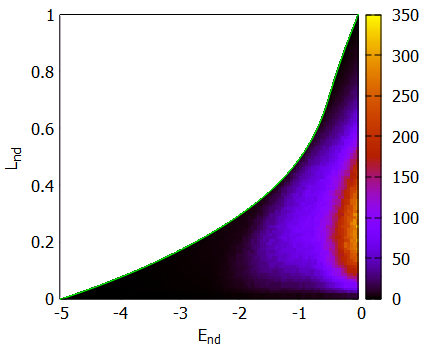
\includegraphics[width=0.532\textwidth]{data/CL_INIT_100_100_sun.png}};
	\draw (8, 0) node[inner sep=0] {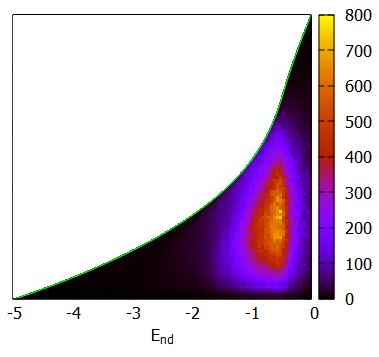
\includegraphics[width=0.463\textwidth]{data/CH_INIT_100_100_sun.png}};
	\draw (-0.8, 1.8) node {$\cfrac{dc^+_{\chi}(t = 0)}{dEdL}$};
	\draw (7.2, 1.8) node {$\cfrac{dc^+_{\chi^*}(t = 0)}{dEdL}$};
\end{tikzpicture}
\caption{ Распределение скорости захвата $\chi$ (слева) и $\chi^*$ (справа), $m_{\chi} = 100 \, \text{ГэВ}$, $\delta = 100 \, \text{кэВ}$}
\label{plot:C_L_100_100}
\end{figure}

\begin{figure}[!h]
	\begin{center}
		\begin{tikzpicture}
			\begin{axis}[
				xscale = 1.6,
				yscale = 1.0,
				xlabel = $r_{nd}$,
				ylabel = $\frac{dc^+_i}{dr}$,
				legend style={at = {(0.56,0.6)},
					anchor = south,legend cell align=right}
				]
				\addplot [color = red, thick] table
				{data/CL_R_INIT_100_100.txt};
				
				\addplot [color = blue, thick] table 
				{data/CH_R_INIT_100_100.txt};
				\legend{$\chi$, $\chi^*$}
			\end{axis}
		\end{tikzpicture}
		\caption{Распределение по радиусу захваченных частиц, $m_{\chi} = 100 \,  \text{ГэВ}$, $\delta = 100 \, \text{кэВ}$}
		\label{plot:r_distrib_100_100}
	\end{center}	
\end{figure}

\section{Результаты численного моделирования термализации}

Приведем результаты моделированния для массы частицы $m_{\chi} = 100 \, \text{кэВ}$, и $\delta = 100 \, \text{кэВ}$ на Солнце. Начальное распределение захваченных частиц по энергии-моменту изображено рисунке \ref{plot:C_L_100_100}, а распределение по радиусу на рисунке \ref{plot:r_distrib_100_100}

Изобразим также матрицу соударений ($s_{ij}$ из \ref{eq:evol_compt}). Для этого построим графики зависимости суммарной вероятности соударений от энергии и момента.

\begin{figure}[!h]
\begin{tikzpicture}
	\draw (0, 0) node[inner sep=0] {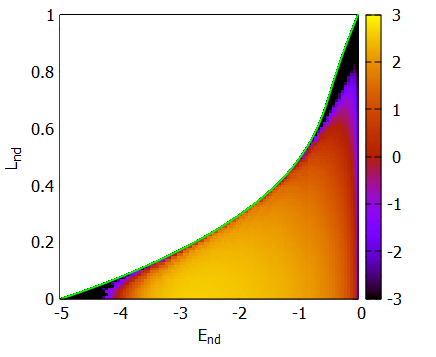
\includegraphics[width=0.545\textwidth]{data/L-.png}};
	\draw (8, 0) node[inner sep=0] {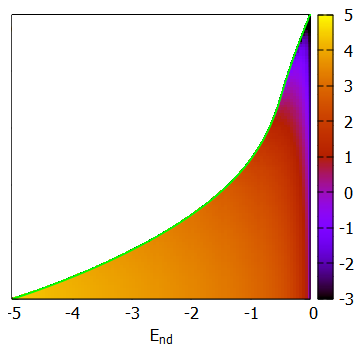
\includegraphics[width=0.455\textwidth]{data/H-.png}};
	\draw (-0.8, 1.8) node {$\lg{(\sum_i s_{ij} \chi \rightarrow \chi^*)}$};
	\draw (7.2, 1.8) node {$\lg{(\sum_i s_{ij} \chi^* \rightarrow \chi)}$};
\end{tikzpicture}
\label{plot:C_LH_minus}
\caption{Вероятность соударений (десятичный логарифм), $m_{\chi} = 100 \, \text{ГэВ}$, $\delta = 100 \, \text{кэВ}$}
\end{figure}

Вероятность рассеяния для тяжелой частиы $\chi^* \rightarrow \chi$ наибольшая при низких энергиях, при которых наибольшая часть траектории находится в наиболее плотной части Солнца. Наименьшие значения вероятность соударения принимает при высоких энергиях и низких моментах импульса, поскольку траектории находятся в наиболее разреженных слоях Солнца, где вероятность рассеяния минимальна. Более того, значительная часть траекторий при этих энергиях и импульсах находится за пределами Солнца, где рассеяния нет.
Для более легкой частицы вероятность рассеяния в тжелую имеет аналогичный вид, однако в зоне с низкими энергиями устремляется к нулю, так как реакция $\chi \rightarrow \chi^*$ имеет порог.

Ниже приведены распределения по энергии-моменту решения $y$ уравнения \ref{eq:solver_y}. При этом рассматривается распределение $y$ во временах $10^{-6}T_{\odot}$, $10^{-4}T_{\odot}$ и $T_{\odot}$, где $T_{\odot}$ время жизни Солнца. 


\begin{figure}[h!]
	\centering
\begin{tikzpicture}
	\draw (0, 0) node[inner sep=0] {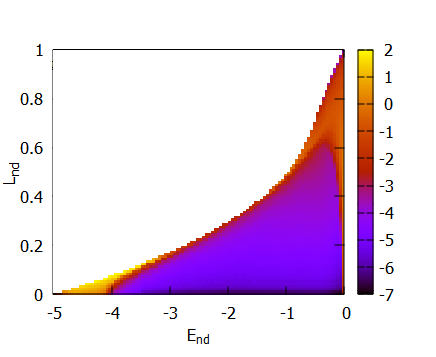
\includegraphics [width=0.54\textwidth] {data/CL_1e-6_100_100.png}};
	\draw (8, 0) node[inner sep=0] {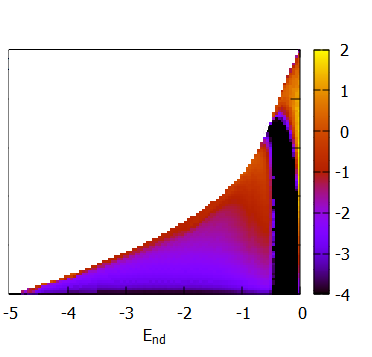
\includegraphics [width=0.46\textwidth] {data/CH_1e-6_100_100.png}};
	\draw (-0.8, 1.8) node {$lg(\frac{dy_{\chi^*}}{dEdL})(t = 10^{-6}T_{\odot})$};
	\draw (7.2, 1.8) node {$lg(\frac{dy_{\chi}}{dEdL})(t = 10^{-6}T_{\odot})$};
\end{tikzpicture}
\begin{tikzpicture}
	\draw (0, 0) node[inner sep=0] {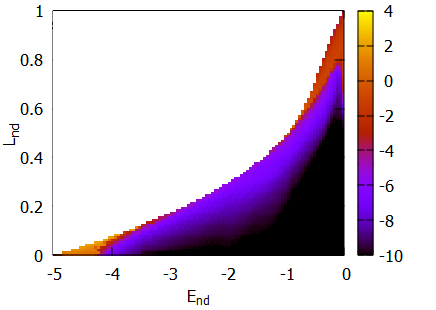
\includegraphics [width=0.54\textwidth] {data/CL_4_100_100.png}};
	\draw (8, 0) node[inner sep=0] {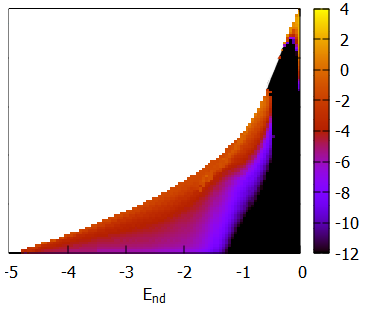
\includegraphics [width=0.46\textwidth] {data/CH_4_100_100.png}};
	\draw (-0.8, 1.8) node {$lg(\frac{dy_{\chi^*}}{dEdL})(t = 10^{-4}T_{\odot})$};
	\draw (7.2, 1.8) node {$lg(\frac{dy_{\chi}}{dEdL})(t = 10^{-4}T_{\odot})$};
\end{tikzpicture}	
\begin{tikzpicture}
	\draw (0, 0) node[inner sep=0] {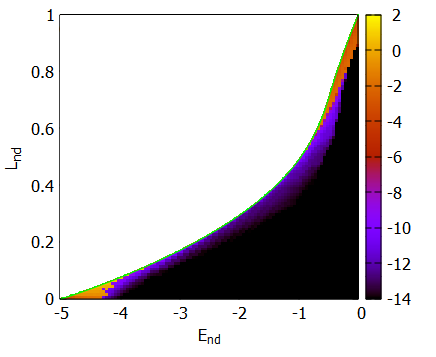
\includegraphics [width=0.54\textwidth] {data/L_1.png}};
	\draw (8, 0) node[inner sep=0] {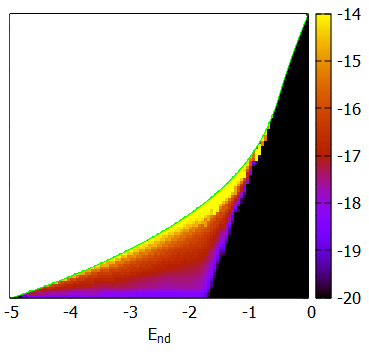
\includegraphics [width=0.46\textwidth] {data/H_1.png}};
	\draw (-0.8, 1.8) node {$lg(\frac{dy_{\chi^*}}{dEdL})(t = T_{\odot})$};
	\draw (7.2, 1.8) node {$lg(\frac{dy_{\chi}}{dEdL})(t = T_{\odot})$};
\end{tikzpicture}
\label{plot:C_LH_evol}
\caption{Эволюция $y$ из \ref{eq:solver_y} $\chi$ (слева) и $\chi^*$ (справа), $m_{\chi} = 100 \, \text{ГэВ}$, $\delta = 100 \, \text{кэВ}$}
\end{figure}

Динамика количества частиц и величины $y$ рассмотрена на графике \ref{plot:n_t} в случае, когда изначально в гало присутствует только легкаяя компонента, и захватывается только тяжелая. За время $0.3T_{\odot}$ почти вся тяжелая компонента $y_{\chi}$ превращается в легкую, выходя на предельный уровень. Полное количество тяжелых частиц остается неизменным, а число легких частиц начинает расти линейно.


\begin{figure}[!h]
	\begin{center}
		\begin{tikzpicture}
			\begin{groupplot}[group style={ group size=2 by 1}]
				\nextgroupplot[
				legend style={at ={(0.9,0.9)}},
				xmax = 0.3,
				xtick distance=0.1,
				xlabel = {$\frac{t}{10^{-8}T_{\odot}}$}
				]
				\addplot [color = blue, thick] table[x index=0,y index=1] 
				{data/C_L_R_ev/out_8_10_n.dat};
				\addplot [color = red, thick] table[x index=0,y index=2] 
				{data/C_L_R_ev/out_8_10_n.dat};
				\legend{$y_{\chi}$, $y_{\chi*}$}
				
				\nextgroupplot[
				legend style={at ={(0.9,0.9)}},
				xlabel = {$\frac{t}{10^{-8}T_{\odot}}$},
				xmax = 0.3,
				xtick distance=0.1
				]
				\addplot [color = blue, thick] table[x index=0,y index=3] 
				{data/C_L_R_ev/out_8_10_n.dat};
				\addplot [color = red, thick] table[x index=0,y index=4] 
				{data/C_L_R_ev/out_8_10_n.dat};
				\legend{$N_{\chi}$, $N_{\chi*}$}
			\end{groupplot}
		\end{tikzpicture}
		\caption{Эволюция числа частиц для $m_{\chi} = 100 \, text{ГэВ}$, $\delta = 100 \, \text{кэВ}$}
		\label{plot:n_t}
	\end{center}	
\end{figure}

\begin{figure}[!h]
	\begin{center}
		\begin{tikzpicture}
			\begin{groupplot}[group style={ group size=2 by 1}]
				\nextgroupplot[
				legend style={at ={(0.9,0.9)}},
				xmax = 0.3,
				xtick distance=0.1]
				\addplot [color = blue, thick] table
				{data/C_L_R_ev/CL_R_1_8.txt};
				\addplot [color = red, thick] table
				{data/C_L_R_ev/thermal.txt};
				
				\legend{$\frac{dy}{dr}(t = 10^{-8}T_{\odot})$, Термальное}
				\nextgroupplot[
				legend style={at ={(0.9,0.9)}},
				xmax = 0.3,
				xtick distance=0.1]
				\addplot [color = blue, thick] table
				{data/C_L_R_ev/CL_R_1.txt};
				\addplot [color = red, thick] table
				{data/C_L_R_ev/thermal.txt};
				\legend{$\frac{dy}{dr}(t = T_{\odot})$, Термальное}
			\end{groupplot}
		\end{tikzpicture}
		\caption{Распределение частиц по радиусу, сравнение с термальным для $m_{\chi} = 100 \, \text{ГэВ}$, $\delta = 100 \, \text{кэВ}$}
		\label{plot:r_distrib}
	\end{center}	
\end{figure}
%Therm density

На рисунке \ref{plot:r_distrib} изобразим распределение частиц темной материи по радиусу в моментах времени $10^{-8}T_{\odot}$ и $T_{\odot}$. Распределение сдвигается в сторону термального (\ref{eq:therm_dens}), однако это распределение не достигается. В результате концентрация неупругой темной материи ниже, чем при термальном равновесии, что ведет к уменьшению темпа аннигиляции и большего времени достижения равновесия в уравнении \ref{eq:evolve_big}
 
\section{Ограничения на сечение}

Решив линейное уравнение эволюции, мы получаем количество частиц и темп аннигиляции $\Gamma_t$ в момент времени $T_{\odot}$ для $\sigma_0$ (мы выбрали $\sigma_0 = 10^{-42} \text{см}^3$). Важным соотношением будет величина 
\begin{equation}
	\cfrac{\Gamma_t}{C}
\end{equation}
где $C$ --- скорость захвата. Если эта величина много больше единицы, то уравнение \ref{eq:evolve_big} пришло к равновесию, и темп аннигиляции равен скорости захвата. Если же это соотношение сильно меньше единицы, то аннигиляция определяется квадратичным слагаемым $AN^2$. На графиках ниже мы изобразим это соотношение в зависимости от $\delta$ для масс $100$ и $1000$ ГэВ.

\begin{figure}[!h]
	\begin{center}
		\begin{tikzpicture}[scale = 0.9]
			\begin{groupplot}[group style={ group size=2 by 1}]
				\nextgroupplot[
				legend style={at ={(0.9,0.9)}},
				ymode = log,
				xlabel = {$\delta, \text{кэВ}$},
				ylabel = {$\frac{\Gamma_{0}}{C_0}$},
				title = {$\frac{\Gamma_{0}}{C_0}, m_{\chi} = 100 ГэВ$}
				]
				\addplot [color = red, thick] table[x index=0,y index=5] 
				{data/cons/C_A_100GeV.txt};
				\addplot [color = blue, thick] table[x index=0,y index=6] 
				{data/cons/C_A_100GeV.txt};
				\legend{$n_{\chi^*}/n_{\chi}= 0$,
						$n_{\chi^*}/n_{\chi}= 1$}
				
				\nextgroupplot[
				legend style={at ={(0.9,0.9)}},
				ymode = log,
				ytick pos=right,
				title = {$\frac{\Gamma_{0}}{C_0}, m_{\chi} = 1000 ГэВ$},
				xlabel = {$\delta, \text{кэВ}$}
				]
				\addplot [color = red, thick] table[x index=0,y index=5] 
				{data/cons/C_A1000GeV.txt};
				\addplot [color = blue, thick] table[x index=0,y index=6] 
				{data/cons/C_A1000GeV.txt};
				\legend{$n_{\chi^*}/n_{\chi}= 0$,
					$n_{\chi^*}/n_{\chi}= 1$}
			\end{groupplot}
		\end{tikzpicture}
		\caption{Отношение аннигиляции к захвату слева $m_{\chi} = 100 \, \text{ГэВ}$, справа ---  $m_{\chi} = 1000 \, \text{ГэВ}$ при сечении рассеяния на протоне $\sigma_{0} = 10^{-42} \,\text{см}^2$}
		\label{plot:A_C}
	\end{center}	
\end{figure}

В конечном итоге, скорость аннигиляции равна
\begin{equation}
	\Gamma_{ann} = C \cdot \tanh^2{\sqrt{\cfrac{\Gamma_t}{C}}} = 
	\cfrac{\sigma_{\chi p}}{\sigma_0} \cdot {C_0} 
	\tanh^2{ \sqrt{\cfrac{\Gamma_0}{C_0} \cfrac{\sigma_{\chi p}}{\sigma_0}}}
	\label{eq:Gamma_ann}
\end{equation}
где $C_0$ и $\Gamma_0$ --- скорость захвата и темп аннигиляции на момент времени $T_{\odot}$, вычисленные в результате решения линейного уравнения эволюции при сечении рассеяния на протоне, равное $\sigma_{0}$ (мы брали $10^{-42}\,\text{см}^2$). Исходя из ограничений IceCube \cite{Aartsen_2017} на число аннигиляций $\Gamma_{ann}$, мы получим ограничение на сечение $\sigma_{\chi p}$, обращая \ref{eq:Gamma_ann}. Для этого будем использовать ограничения на $\Gamma_{ann}$, полученную одельно для каналов аннигиляции: $\tau^+\tau^-$ и $W^+W^-$. Приведем результаты для масс 100 и 1000 ГэВ в предельных случаях, когда в гало нет тяжелой фракции темной материи ($n_{\chi^*}/n_{\chi}= 0$) и когда она распределена поровну ($n_{\chi^*}/n_{\chi}= 1$)

\begin{figure}[!h]
	\begin{center}
		\begin{tikzpicture}
			\begin{axis}[
				scale = 1.7,
				ymode = log,
				%ymin = 1e-1,
				xlabel = {$\delta, \text{кэВ}$},
				%xmax = 500,
				%xlabel shift = {(10,-10)},
				%xtick distance=100,
				title = {$\sigma_{\chi p}, m_{\chi} = 100 \,\text{ГэВ}$},
				%title style={at = {(0.36,1.0)}},
				ylabel = {$\sigma_{\chi p}, \text{см}^2$},
				ylabel style = {yshift = 20pt}, 
				legend style={at = {(0.5,0.94)}}
				]
				
				\addplot [color = red, thick] table [x index=0,y index=6] {data/cons/tau_100GeV.txt};
				\addplot [color = orange, thick] table [x index=0,y index=5] {data/cons/W_100GeV.txt};
				\addplot [color = blue, thick] table [x index=0,y index=5] {data/cons/tau_100GeV.txt};
				\addplot [color = green, thick] table [x index=0,y index=6] {data/cons/W_100GeV.txt};
				\addplot [dashed, color = purple,thick,samples=2] coordinates  {(0,0.8*1e-43) (300,0.8*1e-43)};
					\addplot [dashed, color = gray,thick,samples=2] coordinates  {(0,3*1e-43) (300,3*1e-43)};
				\legend{{$n_{\chi^*}/n_{\chi}= 0, \tau^+\tau^-$},
					{$n_{\chi^*}/n_{\chi}= 0, W^+W^-$},
					{$n_{\chi^*}/n_{\chi}= 1, \tau^+\tau^-$},
					{$n_{\chi^*}/n_{\chi}= 1, W^+W^-$},
					 {Упругое, $\tau^+\tau^-$},
					 {Упругое, $W^+W^-$}}
			\end{axis}
		\end{tikzpicture}		
		\caption{Ограничения на сечение рассеяния с протоном $\sigma_{\chi p} $ при $m_{\chi} = 100 \, \text{ГэВ}$, пунктирными линиями обозначенны ограничения на упругое сечение для каналов $\tau^+\tau^-$ (серый) и $W^+W^-$ (фиолетовый) из \cite{Aartsen_2017}} 
		\label{plot:constrains_100GeV}
	\end{center}	
\end{figure}
\begin{figure}[!h]
	\begin{center}
		\begin{tikzpicture}
			\begin{axis}[
				scale = 1.7,
				ymode = log,
				ymin = 1e-44,
				xlabel = {$\delta, \,\text{кэВ}$},
				xmax = 350,
				%xlabel shift = {(10,-10)},
				%xtick distance=100,
				title = {$\sigma_{\chi p}, m_{\chi} = 1000 \, \text{ГэВ}$},
				title style={at = {(0.36,1.0)}},
				ylabel = {$\sigma_{\chi p}, \text{см}^2$},
				ylabel style = {yshift = 20pt}, 
				legend style={at = {(0.46,0.98)}}
				]
				
				\addplot [color = red, thick] table [x index=0,y index=6] {data/cons/tau_1000GeV.txt};
				\addplot [color = orange, thick] table [x index=0,y index=6] {data/cons/W_1000GeV.txt};
				\addplot [color = blue, thick] table [x index=0,y index=5] {data/cons/tau_1000GeV.txt};
				\addplot [color = green, thick] table [x index=0,y index=5] {data/cons/W_1000GeV.txt};
				\addplot [dashed, color = purple,thick,samples=2] coordinates  {(0,2*1e-44) (300,2*1e-44)};
				\addplot [dashed, color = gray,thick,samples=2] coordinates  {(0,7*1e-44) (300,7*1e-44)};
				\legend{{$n_{\chi^*}/n_{\chi}= 0, \tau^+\tau^-$},
					{$n_{\chi^*}/n_{\chi}= 0, W^+W^-$},
					{$n_{\chi^*}/n_{\chi}= 1, \tau^+\tau^-$},
					{$n_{\chi^*}/n_{\chi}= 1, W^+W^-$},
					{Упругое, $\tau^+\tau^-$},
					{Упругое, $W^+W^-$}}
			\end{axis}
		\end{tikzpicture}
		\caption{Ограничения на сечение рассеяния с протоном $\sigma_{\chi p} $ при $m_{\chi} = 1000 \, \text{ГэВ}$, пунктирными линиями обозначенны ограничения на упругое сечение для каналов $\tau^+\tau^-$ (серый) и $W^+W^-$ (фиолетовый) из \cite{Aartsen_2017}}
		\label{plot:constrains_1000GeV}
	\end{center}	
\end{figure}

